\chapter{Reti neurali ricorrenti (RNN)}\label{ch-20}

Questa è un'introduzione leggera alle \textbf{reti neurali ricorrenti}
(RNN), che saranno approfondite nei corsi ISPR e CNS. Finora le reti
erano \textbf{feedforward} (direzione input → output) e lavoravano su
\textbf{vettori}. Le RNN aggiungono \textbf{connessioni di feedback}
(cicli) nella topologia: la presenza di auto-connessioni dà alla rete
\textbf{proprietà dinamiche} e una \textbf{memoria} (uno stato) delle
computazioni passate. Questo estende la capacità rappresentativa del
modello all'elaborazione di \textbf{sequenze} (e di dati strutturati).
Le RNN sono anche biologicamente plausibili: le reti neurali biologiche
sono ricorrenti.

\section{Perché i dati sequenziali}\label{perchuxe9-i-dati-sequenziali}

Servono modelli per sequenze quando l'uscita dipende dalla
\textbf{storia degli input} (ad esempio nel tempo: modelli dinamici), o
quando il dominio è fatto di \textbf{sequenze di lunghezza variabile}:

\begin{itemize}
\tightlist
\item
  processi dinamici, elaborazione di segnali (filtri, controllo),
  robotica;
\item
  \textbf{linguaggio}: riconoscimento del parlato, NLP, linguaggi
  formali, information retrieval;
\item
  visione e ragionamento su eventi temporali;
\item
  \textbf{serie temporali}: previsioni finanziarie, elaborazione di
  segnali;
\item
  genomica e proteomica (bioinformatica): ad esempio predire la
  struttura di una proteina dalla sequenza di amminoacidi;
\item
  riconoscimento di attività umane da dati di sensori.
\end{itemize}

Le RNN (e gli approcci collegati) sono state il riferimento per
l'elaborazione di sequenze, con risultati allo stato dell'arte nel
\textbf{riconoscimento del parlato} e nell'\textbf{elaborazione del
testo} (traduzione automatica\ldots), ma anche per applicazioni
``divertenti'' come la composizione musicale e la generazione di testo e
parlato.

\section{Dai dati piatti ai dati
strutturati}\label{dai-dati-piatti-ai-dati-strutturati}

Finora i dati erano \textbf{piatti} (vettori). I dati
\textbf{strutturati} sono sequenze, alberi, grafi, dati
multi-relazionali: stringhe, proteine, serie temporali, piccole
molecole, reti.

\subsection{Il nuovo dominio: sequenze e
trasduzioni}\label{il-nuovo-dominio-sequenze-e-trasduzioni}

\begin{itemize}
\tightlist
\item
  \textbf{Dati}: sequenze discrete di \textbf{vettori} (con un ordine
  seriale, ad esempio il tempo), di lunghezza variabile. Ogni elemento
  \(\mathbf{l}_t\) è un vettore (es.
  \(\mathbf{l}_t = [1, 0, 1, 0{,}7]\)).
\item
  \textbf{Task}: una \textbf{trasduzione} nel dominio sequenziale, cioè
  una mappatura \emph{sequenza di input → valore o sequenza di output}.
\end{itemize}

\begin{figure}[htbp]
\centering
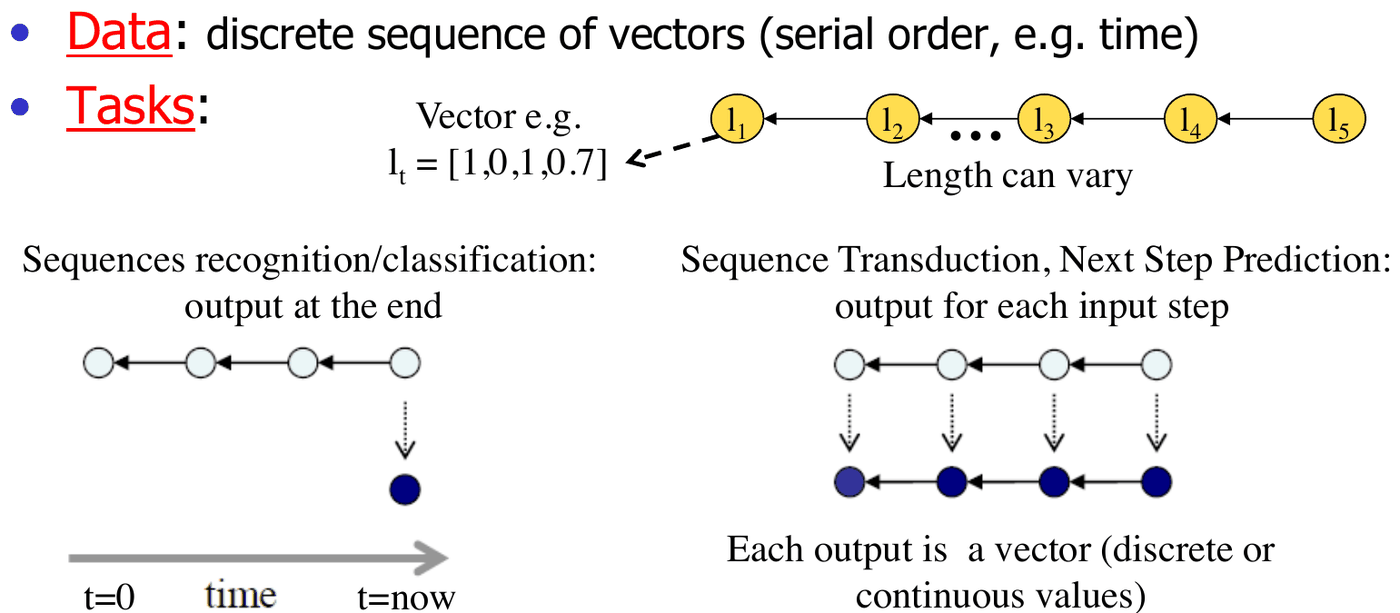
\includegraphics[width=0.80\linewidth,height=0.42\textheight,keepaspectratio]{images/20-rnn_trasduzioni.png}
\caption{Riconoscimento/classificazione di sequenze (uscita alla fine) e
trasduzione di sequenze (uscita a ogni passo).}
\end{figure}

\begin{figure}[htbp]
\centering
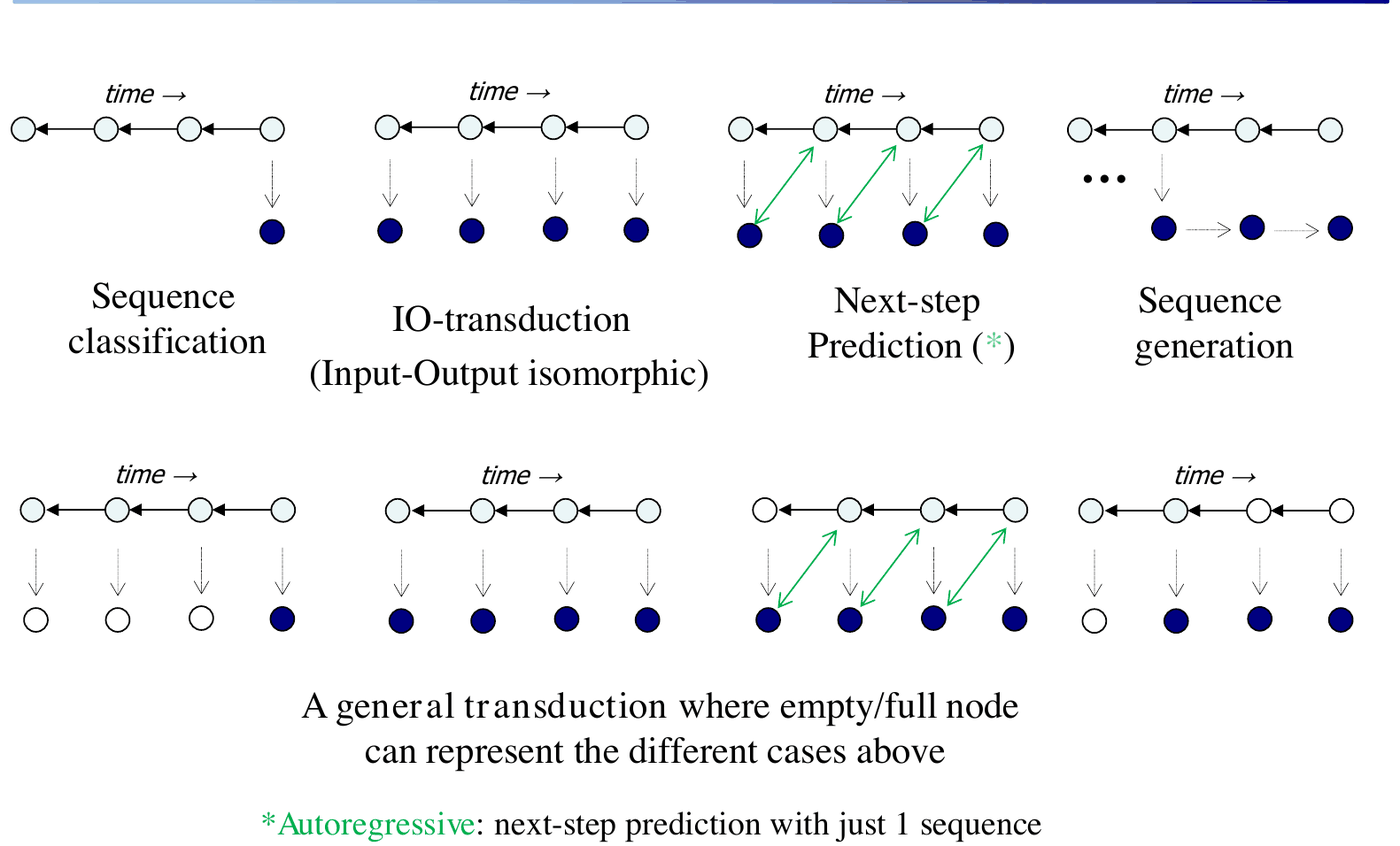
\includegraphics[width=0.80\linewidth,height=0.42\textheight,keepaspectratio]{images/20-rnn_tipi-trasduzione.png}
\caption{Tipi di trasduzione: classificazione di sequenze, trasduzione IO
isomorfa (un'uscita per ogni input), predizione del passo successivo,
generazione di sequenze. La predizione autoregressiva usa una sola
sequenza.}
\end{figure}

\section{La memoria nelle reti
neurali}\label{la-memoria-nelle-reti-neurali}

L'obiettivo è che l'uscita dipenda dagli input \textbf{precedenti}.

\subsection{Approccio 1: memoria finita
(IDNN)}\label{approccio-1-memoria-finita-idnn}

Il primo approccio è ``spaziale'', a \textbf{memoria finita}: le
\textbf{Input Delay Neural Network} (nella classe delle \emph{Time-Delay
NN}, già viste all'inizio delle CNN). I ritardi sono nelle connessioni e
fanno da memoria dell'input: un \textbf{registro a scorrimento} di
dimensione finita, una \textbf{finestra scorrevole} sulla sequenza. (Le
CNN hanno esteso questa idea alle immagini 2D.)

\begin{figure}[htbp]
\centering
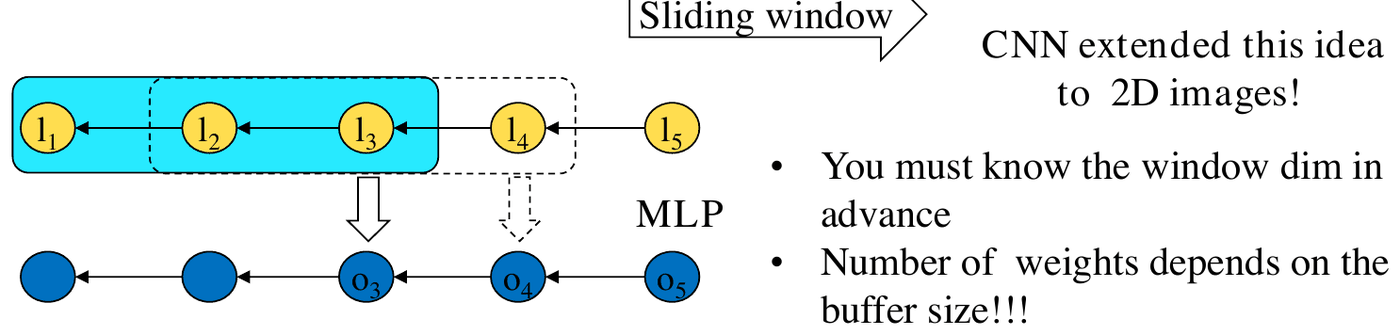
\includegraphics[width=0.74\linewidth,height=0.42\textheight,keepaspectratio]{images/20-rnn_idnn.png}
\caption{IDNN: una finestra scorrevole di dimensione fissa sulla sequenza,
elaborata da un MLP.}
\end{figure}

\begin{itemize}
\tightlist
\item
  La dimensione della finestra va \textbf{nota in anticipo}.
\item
  Il numero di pesi \textbf{dipende dalla dimensione del buffer}.
\item
  Se il buffer contiene abbastanza informazione, si risolve il problema
  con un normale addestramento di MLP (ad esempio NETtalk, 1988).
\end{itemize}

\subsection{Approccio 2: unità
ricorrenti}\label{approccio-2-unituxe0-ricorrenti}

Un'\textbf{unità neurale ricorrente} ha una connessione di feedback (un
\emph{self-loop}) e usa sia l'input corrente sia l'informazione di
\textbf{stato}: \[
x(t) = \tau\big(\mathbf{l}(t), x(t-1)\big) = f\big(\mathbf{w}^T\mathbf{l}(t) + \hat{w}\,x(t-1) + \theta\big), \qquad x(0) = 0,
\] dove \(\mathbf{l}(t)\) è l'input (etichetta) al tempo \(t\), \(f\) è
l'attivazione (sigmoidale), \(\hat{w}\) è il \textbf{peso ricorrente},
\(\theta\) il bias, e \(x(t-1)\) è lo stato al passo precedente, fornito
da un ritardo unitario \(q^{-1}\). La parte nuova rispetto a un neurone
normale è il termine \(\hat{w}\,x(t-1)\).

\begin{figure}[htbp]
\centering
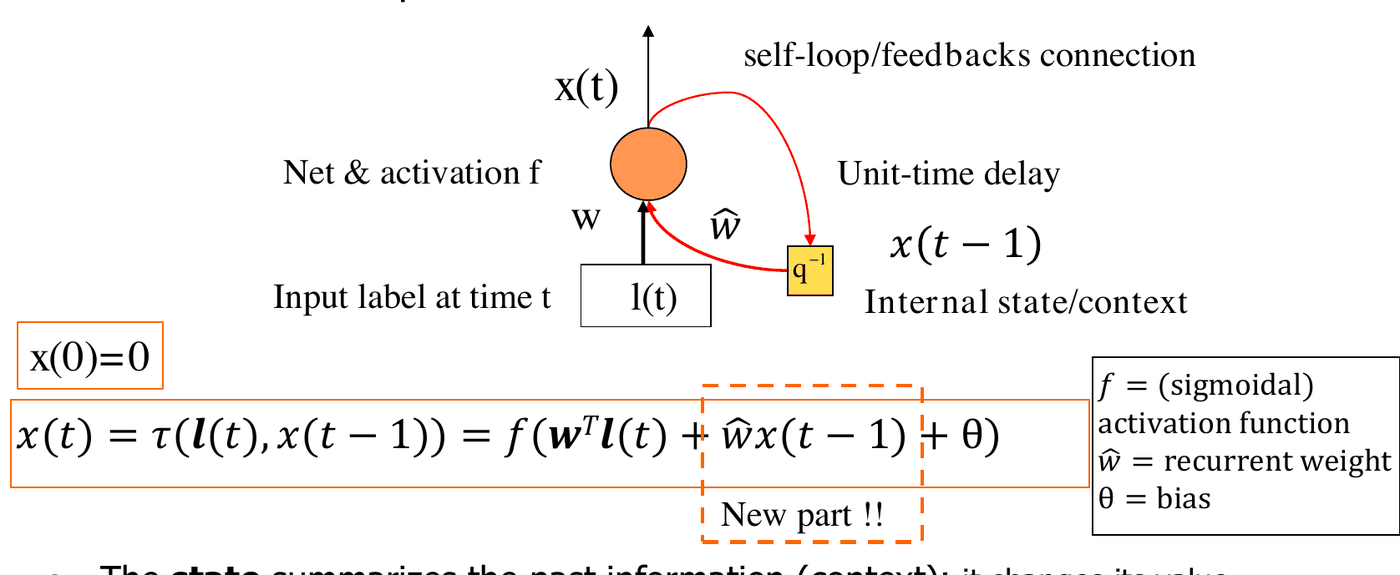
\includegraphics[width=0.86\linewidth,height=0.42\textheight,keepaspectratio]{images/20-rnn_unita-ricorrente.png}
\caption{Un'unità ricorrente: il self-loop con ritardo unitario porta lo stato
precedente come input aggiuntivo.}
\end{figure}

\begin{itemize}
\tightlist
\item
  Lo \textbf{stato} riassume l'informazione passata (il
  \textbf{contesto}): cambia valore seguendo il flusso degli input.
\item
  La \textbf{codifica del passato è adattiva}, perché dipende dai pesi
  liberi del modello.
\end{itemize}

\begin{boxexample}{Esercizio: contare gli ``1''}

Realizzare una RNN con una sola unità (trovando i valori di \(w\) e
\(\hat w\)) che restituisca il numero di ``1'' ricevuti finora in una
sequenza di 0 e 1.

\textbf{Soluzione}: unità lineare con \(w = 1\), \(\hat w = 1\),
\(\theta = 0\), cioè \(x(t) = l(t) + x(t-1)\). Con l'input
\(1, 0, 1, 1, 0, 1\) lo stato vale \(1, 1, 2, 3, 3, 4\): \textbf{lo
stato accumula la somma degli ``1''} ricevuti. La RNN riassume
l'informazione della sotto-sequenza passata, cosa che una IDNN
\textbf{non può fare} per sequenze di lunghezza variabile (la sua
memoria è limitata alla finestra).

\end{boxexample}

\subsection{Sistemi a transizione di
stato}\label{sistemi-a-transizione-di-stato}

In generale, un modello ricorrente è un \textbf{sistema a transizione di
stato}: \[
\begin{cases} \mathbf{x}(t) = \tau\big(\mathbf{x}(t-1), \mathbf{l}(t)\big) \\ \mathbf{y}(t) = g\big(\mathbf{x}(t), \mathbf{l}(t)\big) \end{cases} \qquad \mathbf{x}(0) = \mathbf{0}.
\]

\begin{figure}[htbp]
\centering
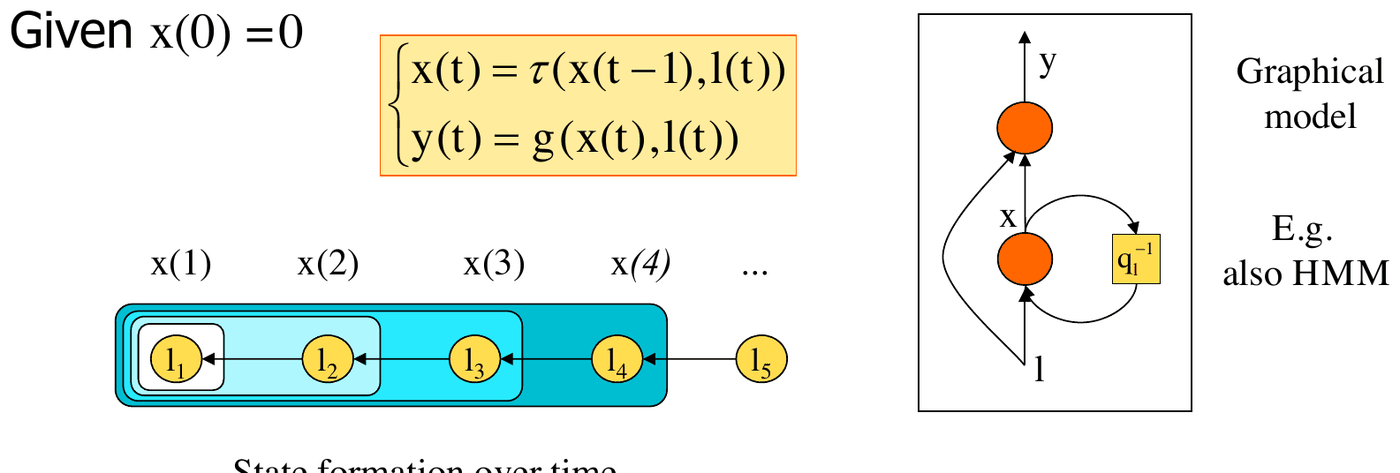
\includegraphics[width=0.80\linewidth,height=0.42\textheight,keepaspectratio]{images/20-rnn_sistema-stati.png}
\caption{Sistema a transizione di stato: lo stato al tempo \(t\) codifica (è un}
\end{figure}

\begin{itemize}
\tightlist
\item
  \(\tau\) è la \textbf{funzione di transizione di stato}
  (\emph{next-state function}), realizzata da una rete neurale.
\item
  Lo stato riassume gli input passati: è una \textbf{codifica}
  (embedding) delle sotto-sequenze.
\item
  Lo stato ha valori \textbf{continui} (reali) (a differenza, ad
  esempio, degli automi o degli HMM, che hanno stati discreti).
\item
  \(\mathbf{x}(t)\) può essere un insieme di stati, per comporre una
  rete di unità ricorrenti.
\end{itemize}

\subsection{Una rete ricorrente (Simple
RNN)}\label{una-rete-ricorrente-simple-rnn}

Con molte unità ricorrenti nascoste si ottiene la \textbf{Simple RNN} di
Elman: ogni unità nascosta riceve l'input e gli stati precedenti di
\textbf{tutte} le unità nascoste (attraverso i ritardi), e uno strato di
uscita (eventuale) produce \(\mathbf{y}(t)\).

\begin{figure}[htbp]
\centering
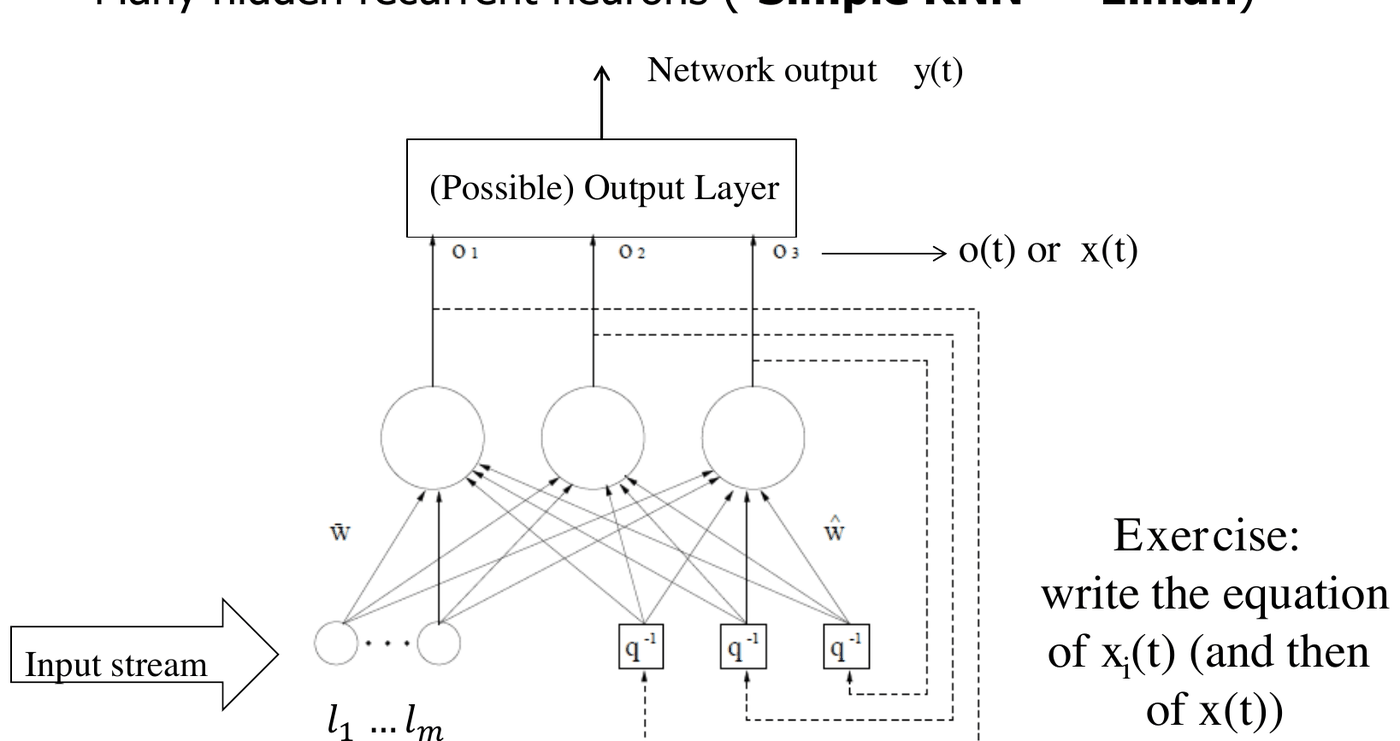
\includegraphics[width=0.86\linewidth,height=0.42\textheight,keepaspectratio]{images/20-rnn_elman.png}
\caption{Una Simple RNN (Elman) con più unità ricorrenti nascoste.}
\end{figure}

\begin{boxexample}{Esercizio: le equazioni}

Per l'unità nascosta \(i\): \[
x_i(t) = f\left(\sum_{j=1}^{m} w_{ij}\,l_j(t) + \sum_{k} \hat w_{ik}\,x_k(t-1) + \theta_i\right),
\] e in forma vettoriale
\(\mathbf{x}(t) = f\big(W\mathbf{l}(t) + \hat W\mathbf{x}(t-1) + \boldsymbol{\theta}\big)\).

\end{boxexample}

\subsection{Proprietà}\label{proprietuxe0}

Anche la semplice RNN è già molto potente:

\begin{itemize}
\tightlist
\item
  è un \textbf{approssimatore universale} di sistemi dinamici non
  lineari;
\item
  è \textbf{Turing-equivalente} (può simulare qualunque automa);
\item
  è un sistema dinamico non lineare (non autonomo), studiabile con la
  teoria dei sistemi dinamici (caos, frattali\ldots).
\end{itemize}

I modelli ricorrenti si basano su tre assunzioni:

\begin{itemize}
\tightlist
\item
  \textbf{Causalità}: l'uscita al tempo \(t_0\) dipende solo dagli input
  ai tempi \(t \le t_0\). È necessaria e sufficiente per avere uno stato
  interno.
\item
  \textbf{Stazionarietà}: invarianza nel tempo (dopo l'addestramento):
  la funzione di transizione \(\tau\) è \textbf{la stessa} in ogni
  istante, indipendentemente dalla lunghezza delle sequenze. È ciò che
  permette di elaborare dati di lunghezza variabile con un modello di
  dimensione fissa.
\item
  \textbf{Adattività}: le funzioni di transizione sono realizzate da
  reti neurali con pesi liberi, quindi \textbf{apprese dai dati}.
\end{itemize}

\section{Apprendimento: l'unfolding}\label{apprendimento-lunfolding}

Si \textbf{srotola} (\emph{unfolding}) nel tempo lo stesso modello lungo
la sequenza di input: si costruisce un MLP feedforward (la \textbf{rete
di codifica}, \emph{encoding network}) equivalente alla RNN sui \(k\)
passi della sequenza, con \textbf{una replica del modello per ogni
passo}. Per la stazionarietà, le repliche \textbf{condividono i pesi}.

\begin{figure}[htbp]
\centering
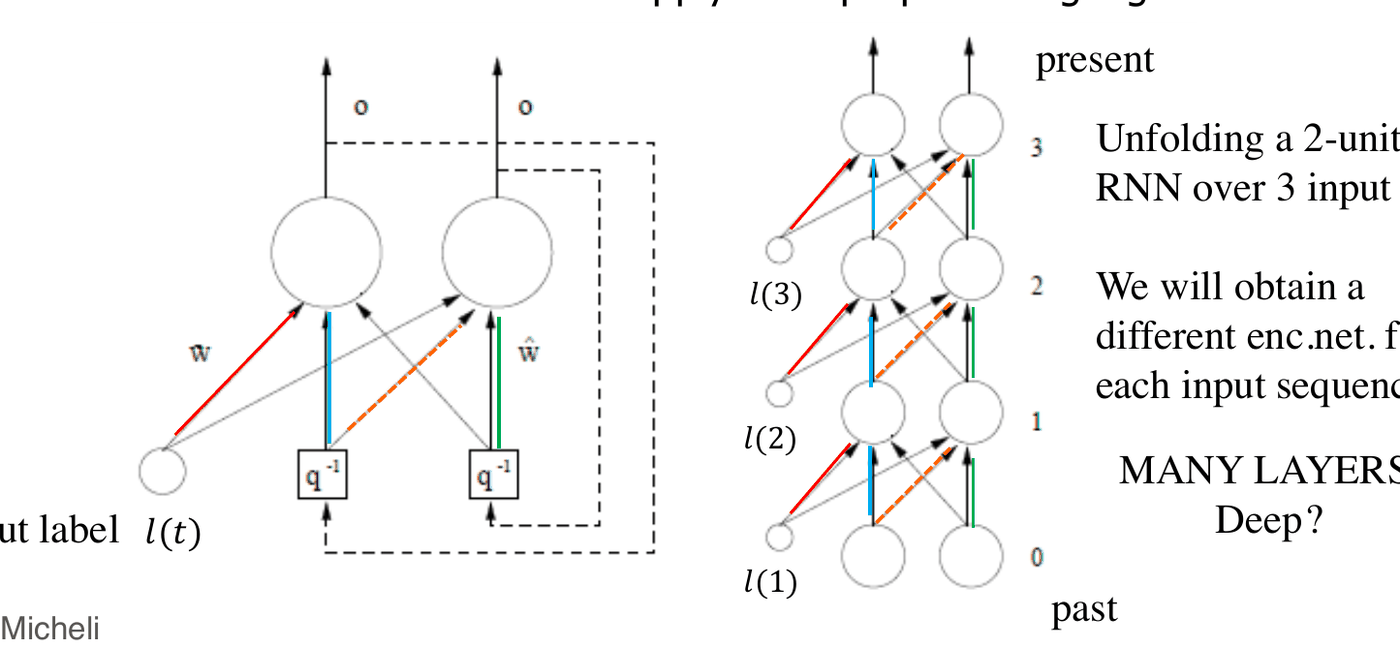
\includegraphics[width=0.74\linewidth,height=0.42\textheight,keepaspectratio]{images/20-rnn_unfolding.png}
\caption{Unfolding di una RNN a 2 unità su 3 passi di input: si ottiene una rete
feedforward a molti strati, diversa per ogni sequenza di input.}
\end{figure}

\begin{boxtip}{Il punto chiave}

Sulla rete di codifica srotolata si può applicare la
\textbf{backpropagation}! Si ottiene una rete diversa per ogni sequenza
di input, con \textbf{molti strati} (tanti quanti i passi): è di fatto
una rete \textbf{profonda}, con pesi condivisi tra gli strati.

\end{boxtip}

Gli algoritmi di apprendimento supervisionato per RNN devono tenere
conto di tutte le transizioni di codifica sviluppate dal modello a ogni
passo:

\begin{itemize}
\tightlist
\item
  \textbf{BPTT} (\emph{Back-Propagation Through Time});
\item
  \textbf{RTRL} (\emph{Real-Time Recurrent Learning}).
\end{itemize}

Calcolano in modo diverso lo stesso gradiente degli errori di uscita
sulla rete srotolata equivalente.

\begin{boxwarning}{Dipendenze a lungo termine}

Poiché la rete srotolata è molto profonda, il \textbf{vanishing
gradient} rende difficile apprendere \textbf{dipendenze a lungo termine}
(quando l'uscita dipende da input molto lontani nel passato).

\end{boxwarning}

\subsection{Modelli avanzati}\label{modelli-avanzati}

È un campo di ricerca in rapida crescita, con molte varianti:

\begin{itemize}
\tightlist
\item
  \textbf{LSTM} (\emph{Long Short-Term Memory}): cercano di risolvere il
  vanishing gradient con \textbf{unità ``gate''} capaci di selezionare
  il flusso del passato e del gradiente. Sono nate per le dipendenze
  \textbf{lunghe}: non sono adatte a serie brevi, quindi, nonostante la
  popolarità, non vanno usate acriticamente;
\item
  \textbf{GRU} (\emph{Gated Recurrent Units}): una LSTM semplificata;
\item
  \textbf{BRNN} (RNN bidirezionali): considerano sia il contesto a
  sinistra sia quello a destra;
\item
  spesso si fondono reti profonde e RNN;
\item
  contro il vanishing gradient: ottimizzatori Hessian-free, tecniche di
  pre-training\ldots{}
\end{itemize}

Sono incluse nelle principali librerie (PyTorch, Keras, Matlab\ldots).
Alcuni dati sulla loro diffusione: nel 2015 le LSTM erano usate in 2
miliardi di telefoni Android e 1 miliardo di iPhone (Siri); nel 2016
quasi il 30\% della potenza di calcolo per l'inferenza dei datacenter di
Google era usato per le LSTM; nel 2017 erano in Alexa e in Facebook (30
miliardi di traduzioni a settimana). Un esempio curioso: generare la
versione \textbf{manoscritta} di un testo predicendo un punto \((x,y)\)
della traiettoria della penna alla volta (Graves, 2013).

\section{Approcci collegati}\label{approcci-collegati}

\begin{itemize}
\tightlist
\item
  SOM e reti non supervisionate per domini sequenziali.
\item
  \textbf{Hidden Markov Model} (modellano la distribuzione di
  probabilità delle transizioni di stato).
\item
  \textbf{Transformer}.
\item
  \textbf{RNN randomizzate}: il \textbf{Reservoir Computing} (ESN,
  \emph{Liquid State Machine}).
\item
  Modelli basati su distanze (string matching), kernel per stringhe,
  inferenza grammaticale, ILP.
\end{itemize}

\subsection{Transformer e attenzione}\label{transformer-e-attenzione}

Un \textbf{transformer} (2017) è un'architettura di deep learning basata
sul meccanismo di \textbf{attenzione multi-head} in parallelo.
L'attenzione permette al modello di \textbf{accedere a qualunque punto
precedente} della sequenza; encoder e/o decoder più reti feedforward
completano l'architettura per scopi diversi.

Lo \textbf{strato di attenzione} pesa tutti gli stati precedenti secondo
una misura di \textbf{rilevanza appresa}, fornendo potenzialmente
informazione anche su token molto lontani. Si è rivelato particolarmente
utile nella traduzione, dove un contesto lontano può essere essenziale
per il significato di una parola. Usato prima per migliorare le RNN, poi
anche da solo (\emph{``Attention is all you need''}). Tutti i token
vengono elaborati \textbf{simultaneamente}, calcolando pesi tra le loro
rappresentazioni (embedding) in strati successivi: sono semplicemente
unità a \textbf{prodotto scalare scalato} tra vettori \emph{query} e
vettori delle parole, che cercano le correlazioni più alte tra le parole
di una frase (ad esempio in ``see that girl'', ``that'' viene associato
a ``girl''). Si applica anche a \emph{patch} di immagini invece che a
parole (\emph{vision transformer}).

\subsection{Reti ricorrenti randomizzate: le Echo State
Network}\label{reti-ricorrenti-randomizzate-le-echo-state-network}

Possiamo sfruttare direttamente questa macchina a stati per codificare
le sequenze, e poi usare l'embedding risultante per imparare la
mappatura di uscita? Sì, \textbf{anche con reti ricorrenti connesse
casualmente con pesi fissi} (non addestrati)! È la classe del
\textbf{Reservoir Computing} (RC): Echo State Network, \emph{liquid
state machine}, \emph{fractal machine} (si veda
\href{18\%20-\%20Reti\%20neurali\%20randomizzate}{18 - Reti neurali
randomizzate}).

\begin{figure}[htbp]
\centering
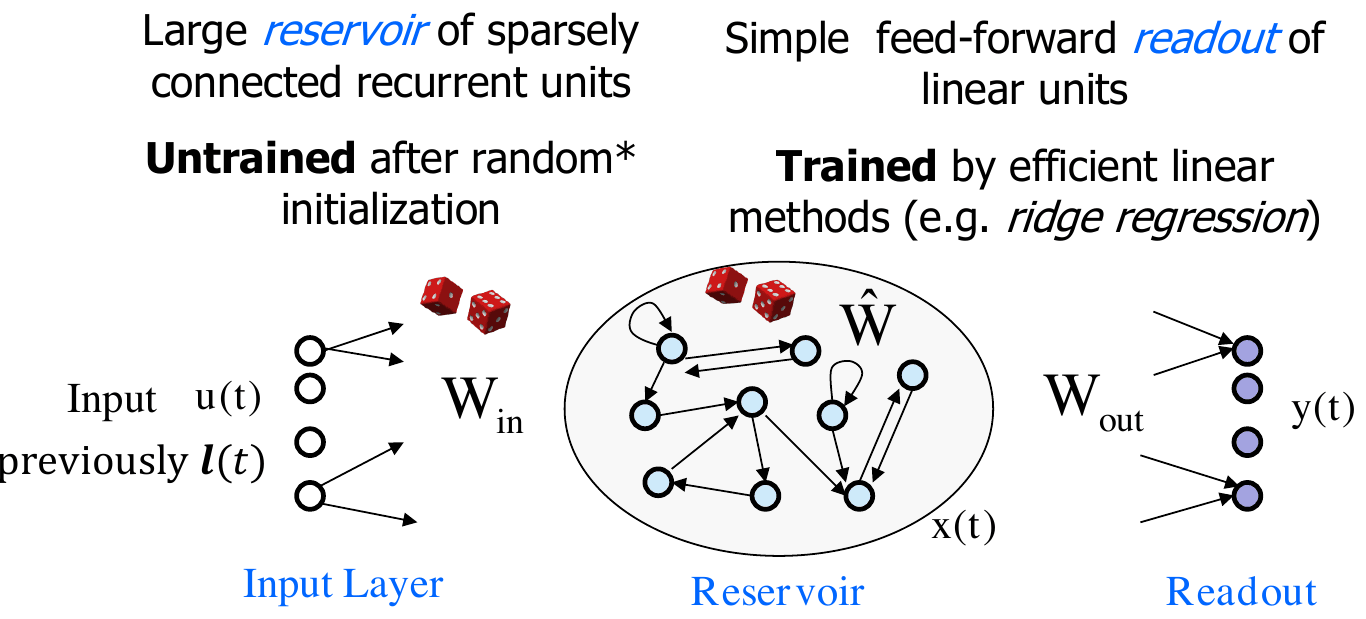
\includegraphics[width=0.80\linewidth,height=0.42\textheight,keepaspectratio]{images/20-rnn_esn.png}
\caption{Una Echo State Network: reservoir casuale non addestrato e readout
lineare addestrato.}
\end{figure}

\begin{boxdefinition}{Echo State Network (ESN)}

Una ESN è composta da: - un grande \textbf{reservoir} di unità
ricorrenti connesse in modo sparso, \textbf{non addestrate} dopo
un'inizializzazione casuale; - un semplice \textbf{readout} feedforward
di unità \textbf{lineari}, addestrato con metodi lineari efficienti (es.
\textbf{ridge regression}).

\textbf{Echo State Property}: la funzione di transizione di stato deve
essere \textbf{contrattiva} (si limita il raggio spettrale dei pesi del
reservoir, cioè si garantisce la stabilità del sistema dinamico). Così
lo stato ricorrente dipende asintoticamente (come un'\,``eco'')
\textbf{solo dalla storia degli input}, e non dalle condizioni iniziali
dello stato.

\end{boxdefinition}

Le ESN sono \textbf{molto efficienti} (nessun addestramento delle unità
ricorrenti) e risolvono bene i task sotto certe condizioni.

\subsubsection{Organizzazione markoviana dello spazio degli
stati}\label{organizzazione-markoviana-dello-spazio-degli-stati}

\begin{figure}[htbp]
\centering
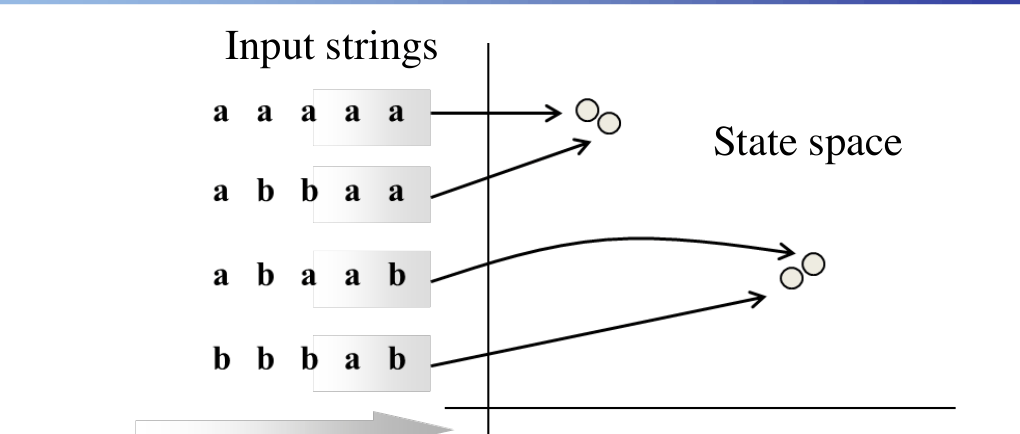
\includegraphics[width=0.54\linewidth,height=0.42\textheight,keepaspectratio]{images/20-rnn_markov.png}
\caption{Il reservoir proietta le sequenze nello spazio degli stati in modo
``markoviano'': sequenze con lo stesso suffisso finiscono vicine.}
\end{figure}

Il reservoir agisce come una \textbf{proiezione} (embedding) delle
sequenze di input nel vettore degli stati \(\mathbf{x}(t)\), e riesce
intrinsecamente a \textbf{discriminare le sequenze in base al suffisso},
senza addestrare i pesi ricorrenti: gli stati sono tanto più vicini
quanto più è lungo il \textbf{suffisso comune} (gli input recenti
contano di più, per la contrattività). Questo rende facile apprendere
task \textbf{markoviani} (anche per le RNN addestrate, ma le ESN sono
molto più efficienti), ed è un \textbf{bias architetturale} che vale
anche per i modelli ricorrenti con apprendimento (Gallicchio, Micheli,
2011).

\textbf{Reservoir Computing profondo.} Si possono impilare più reservoir
(\textbf{DeepESN}, con molti risultati del gruppo CIML di Pisa), unendo
la potenza delle RNN profonde all'efficienza delle ESN. L'organizzazione
a strati mostra vantaggi in termini di \textbf{scale temporali multiple}
e di \textbf{ricchezza delle dinamiche}: nell'analisi in frequenza, gli
strati più alti si concentrano sulle frequenze più basse (scale
temporali più ampie), formando una rappresentazione temporale
gerarchica.

\section{Verso i domini strutturati}\label{verso-i-domini-strutturati}

Si può estendere l'approccio ricorrente agli \textbf{alberi}? Sì: le
\textbf{reti neurali ricorsive} (RecNN). La codifica procede \textbf{dal
basso verso l'alto} (dalle foglie alla radice), e lo stato di ogni
vertice dipende dal suo label e dagli stati dei \textbf{figli}
(estendendo la funzione di transizione a più stati).

\begin{figure}[htbp]
\centering
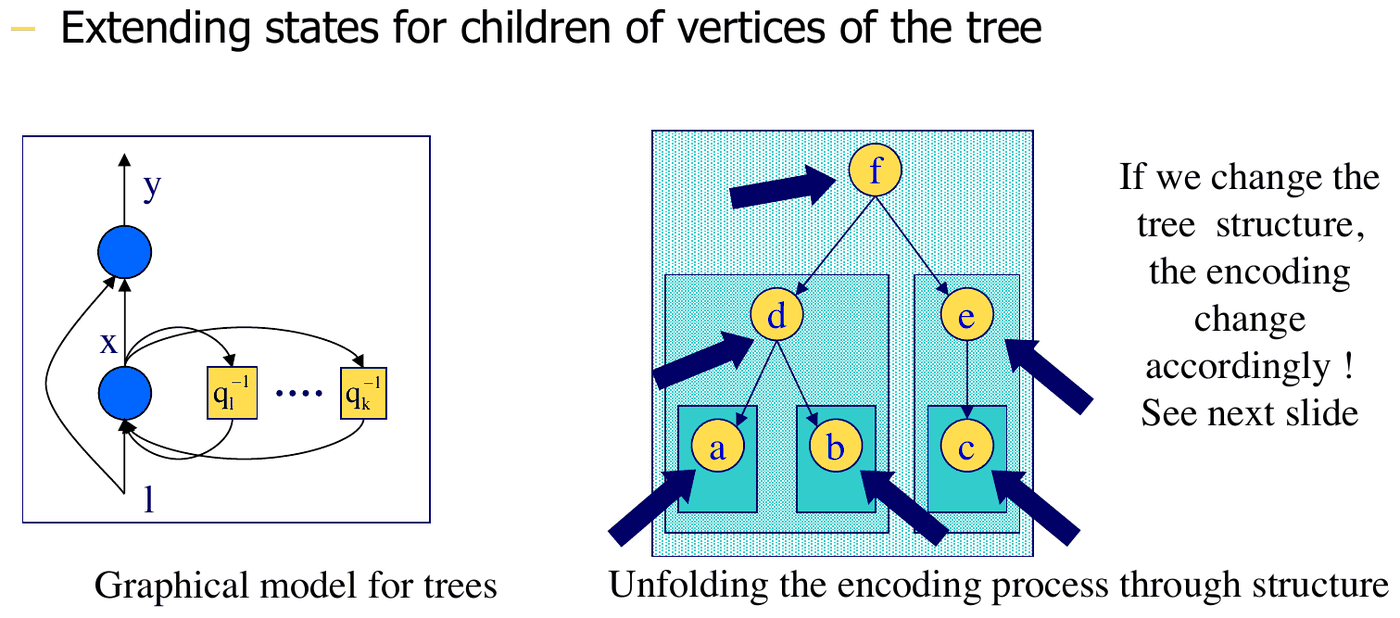
\includegraphics[width=0.74\linewidth,height=0.42\textheight,keepaspectratio]{images/20-rnn_alberi.png}
\caption{Modello grafico per alberi e unfolding della codifica lungo la
struttura: se la struttura dell'albero cambia, la codifica cambia di
conseguenza.}
\end{figure}

\begin{figure}[htbp]
\centering
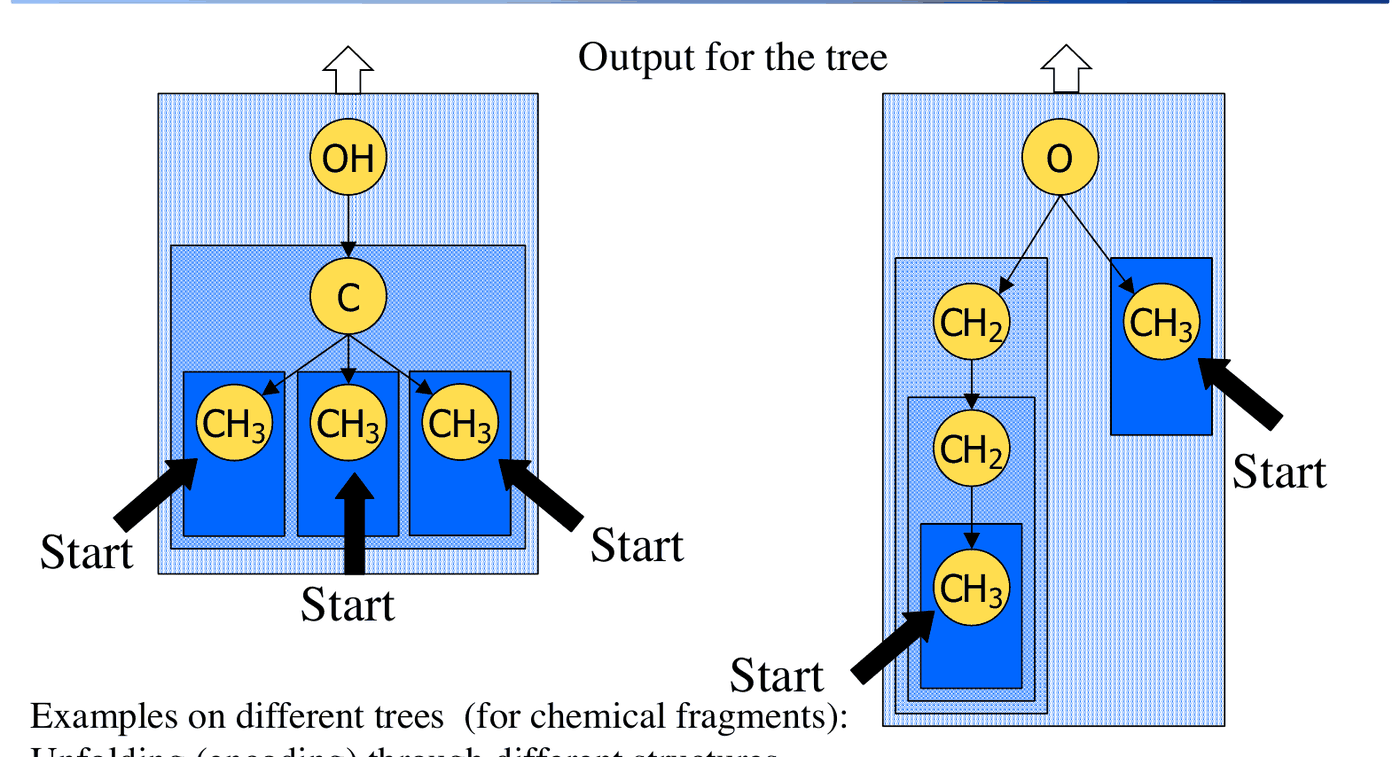
\includegraphics[width=0.74\linewidth,height=0.42\textheight,keepaspectratio]{images/20-rnn_recnn.png}
\caption{Una rete ricorsiva applicata ad alberi diversi (frammenti chimici): le
unità sono le stesse per tutti i vertici di un albero e per tutti gli
alberi del dataset (condivisione dei pesi).}
\end{figure}

\begin{boxabstract}{Sintesi}

Le RNN aggiungono \textbf{stati} e \textbf{feedback} alle reti,
diventando \textbf{sistemi a transizione di stato} capaci di elaborare
sequenze di lunghezza variabile. Si basano su causalità, stazionarietà e
adattività; si addestrano \textbf{srotolandole} nel tempo e applicando
la backpropagation (BPTT, RTRL), ma soffrono di \textbf{vanishing
gradient} sulle dipendenze lunghe (da cui LSTM e GRU). Alternative e
sviluppi: transformer (attenzione), Echo State Network (reservoir
casuale + readout lineare, con un bias markoviano), reti ricorsive per
alberi e grafi.

\end{boxabstract}

\begin{boxquestion}{Possibili domande d'esame}

\begin{itemize}
\tightlist
\item
  Perché servono modelli per dati sequenziali? Cos'è una trasduzione?
\item
  Differenza tra IDNN e RNN; perché una IDNN non può contare gli ``1''
  in sequenze arbitrarie?
\item
  Scrivere l'equazione di un'unità ricorrente e di una Simple RNN.
\item
  Quali sono le assunzioni di causalità, stazionarietà e adattività?
\item
  Cos'è l'unfolding e come permette di usare la backpropagation?
\item
  Cos'è una Echo State Network e cos'è la Echo State Property?
\item
  Come si estendono le RNN agli alberi?
\end{itemize}

\end{boxquestion}
